\section{Summary of Data Sets}\label{sec:data-summary}

In \Cref{tab:dataset-info} we summarize the datasets we use in our paper.

\begin{table}
  \centering
  \caption{Details of the real datasets used in the experiments. The median \(q\) value
    refers to the median of the proportion of ones for the binary features in the data. Note that in the case of \data{housing}, there is
    only a single binary feature.}
  \label{tab:dataset-info}
  \small
  \begin{tabular}{
      l
      S[table-format=4.0]
      S[table-format=4.0]
      l
      l
      S[table-format=1.3,round-mode=places,round-precision=3]
      p{6cm}
    }
    \toprule
    Dataset           & {\(n\)} & {\(p\)} & Response   & Design     & {Median \(q\)} & Description                                                                                                                                                                                                                                                                                 \\
    \midrule

    \data{eunite2001} & 336     & 16      & continuous & mixed      & 0.856143       & Mid-term load forecasting competition dataset (EUNITE 2001) using National Taiwan University's winning approach. Contains 15 features including 7-day historical loads (scaled) with winter-only training data from 1997-1998 to predict January 1999 daily maximum loads \citep{chen2004}. \\

    \addlinespace
    \data{housing}    & 506     & 13      & continuous & mixed      & 0.93083        & Boston housing dataset with information about housing in the Boston area. Response is median value of owner-occupied homes in \$1000s \citep{harrison1978}.                                                                                                                                 \\

    \addlinespace
    \data{triazines}  & 186     & 60      & continuous & mixed      & 0.973118       & Pharmaceutical dataset relating molecular structures of triazine derivatives to their ability to inhibit dihydrofolate reductase \citep{hirst1994,king1995}.                                                                                                                                \\

    \addlinespace
    \data{rhee2006}   & 842     & 361     & continuous & binary     & 0.995249       & HIV-1 drug resistance data with protease and reverse transcriptase mutations as features. Response measures in vitro susceptibility to antiretroviral drugs \citep{rhee2006}.                                                                                                               \\

    \addlinespace
    \data{leukemia}   & 38      & 7129    & binary     & continuous &                & Gene expression data for leukemia patients. Classifies between acute myeloid leukemia (AML) and acute lymphoblastic leukemia (ALL) \citep{golub1999}.                                                                                                                                       \\

    \addlinespace
    \data{australian} & 690     & 14      & binary     & continuous & 0.557246       & Credit approval dataset, originally from the StaLog database. The task is to predict credit approval using a number of different features~\citep{quinlan1987,henery1992}.                                                                                                                  \\

    \addlinespace
    \data{heart}      & 270     & 13      & binary     & mixed      & 0.677778       & Heart disease dataset, originally from the StatLog database. The task is to predict the presence of heart disease from a number of features that have already been selected from a larger set of features~\citep{henery1992}.                                                              \\

    \addlinespace
    \data{a1a}        & 1605    & 123     & binary     & binary     & 0.970093       & Subset of Adult dataset derived from census data. Predicts whether income exceeds \$50,000/year based on census information \citep{becker1996,platt1998}.                                                                                                                                   \\

    \addlinespace
    \data{w1a}        & 2477    & 300     & binary     & binary     & 0.976181       & Derived from web page data, classifying whether pages belong to specific categories \citep{platt1998}.                                                                                                                                                                                      \\

    \bottomrule
  \end{tabular}
\end{table}

We also visualize the distribution of class balance among all the binary features in
\Cref{fig:data-hist-q}. We note that the class imbalance for many of these datasets is
quite severe.

\begin{figure}[htpb]
  \centering
  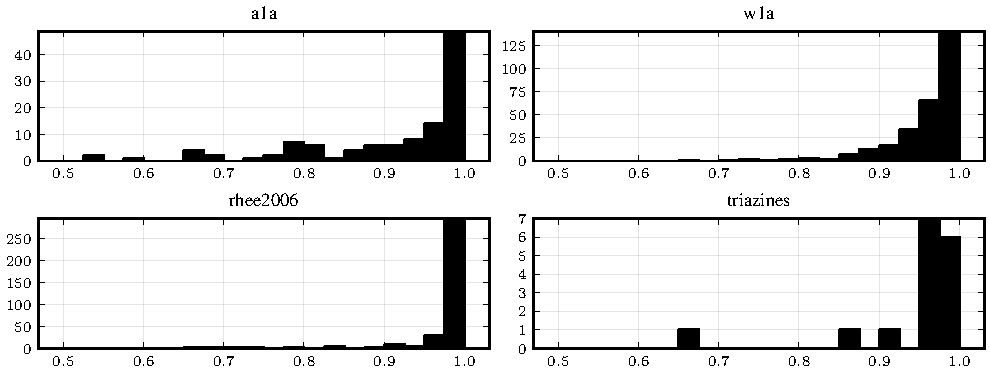
\includegraphics[]{data-hist-q.pdf}
  \caption{%
    Histograms over the distribution of \(q\) (class balance, that is, the
    proportion of ones) for the binary features in each of the datasets
    used in the paper.
  }
  \label{fig:data-hist-q}
\end{figure}

